\subsection{Fixpoint definition for approximations}

We discuss the naive and the fixpoint method based on the example
  depicted in figure \ref{fig:example}.

\begin{figure}
\label{fig:example}
\centering
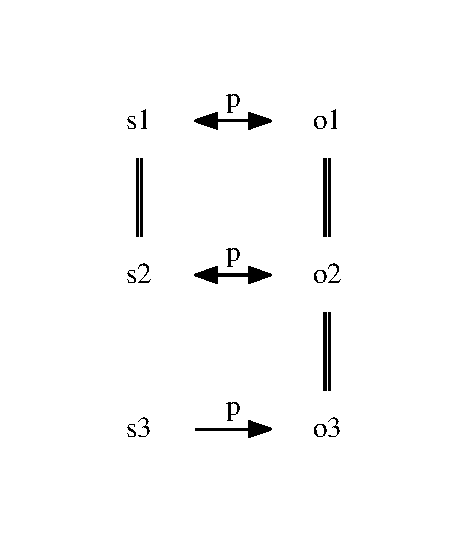
\includegraphics{./img/fixpoint_example}%[width=\columnwidth]
\caption{
  An illustrative example in which we show that defining
  $\underline{\approx}$ in terms of $\indp_{\approx}$ may not be optimal.
  The identity relation is represented with double-lined edges.
}
\end{figure}

%\begin{equation}
%\label{eq:10}
%\approx = \set{\pair{s_1}{s_2},\pair{o_1}{o_2},\pair{o_2}{o_3}}
%\end{equation}

The indiscernibility criteria for this example are shown
  in equation \ref{eq:20}.

\small
\begin{align}
\label{eq:20}
  \indp_{\approx}(\set{s_1,s_2,s_3})
=
  \indp_{\approx}(\set{o_1,o_2})
=
  \setdef{p^n}{\natnum{n}}
\end{align}
\normalsize

Based on the indiscernibility criteria in euqation \ref{eq:20} and
  the definition of the lower approximation
  (def. \ref{def:lower_approximation})
  we derive that the lower approximation for the example
  in figure \ref{fig:example} is empty.

If we change the relation that is used for calculating
  the closures of the predicate and object terms
  in the specification of the discernibility criteria,
  then the results for the lower approximation change.
According to the alternative definition \ref{def:lower_approximation2},
  there are two consistent solutions for the lower approximation:
  \begin{enumerate}
    \item $\lowerapprox_1 = \emptyset$,
          with $\indp_{\lowerapprox_1}(X) = \emptyset$
          for $X$ such that $\card{X} > 1$.
    \item $\lowerapprox_2 = \set{\pair{s_1}{s_2},\pair{o_1}{o_2}}$,
          with $\indp_{\lowerapprox_2}(\set{s_1,s_2,o_1,o_2}) = \setdef{p^n}{\natnum{n}}$
          and $\indp_{\lowerapprox_1}(X) = \emptyset$
          for all other $X$ such that $\card{X} > 1$.
  \end{enumerate}

Both solutions are correct,
  since both conform to the same strictures imposed by the framework.
It may also be reasonable to consider a greater lower approximation
  as more optimal, and the greatest lower approximation as most optimal.

\small
\begin{definition}
\begin{align}
\label{def:lower_approximation2}
  x_1 \lowerapprox x_2
\quad \iff \quad
  \forall_{\pair{y_1}{y_2} \in S_G^2}(\\
        \indp_{\lowerapprox}(\set{y_1,y_2})
      =
        \indp_{\lowerapprox}(\set{x_1,x_2})
    \rightarrow
      y_1 \approx y_2
  )\nonumber
\end{align}
\end{definition}
\normalsize

We have given an example for the lower approximation.
We expect that similar considerations apply to the higher approximation,
  where we maintain that the smallest higher approximation is
  the most optimal one.

